% !TEX root = ../Projektdokumentation.tex
\section{Implementierungsphase} 
\label{sec:Implementierungsphase}

Bevor mit der Implementierung begonnen wurde, wurde ein Iterationsplan erstellt. In diesem wurden die einzelnen Schritte und deren Reihenfolge festgelegt. In jeder Iteration wurde eine spezifische Funktionalität umgesetzt und am Ende der jeweiligen Iteration dem Team präsentiert. Dieses Vorgehen folgt den in Abschnitt \hyperlink{agil}{2.3} beschriebenen Prinzipien der agilen Softwareentwicklung. Der vollständige Iterationsplan befindet sich im \Anhang{app:Iterationsplan}.

\subsection{Implementierung der GitLab Systemhook}
\label{sec:ImplementierungGitlabSystemhook}

Im Rahmen der Implementierung der \hyperlink{GitLab}{\textcolor{AOBlau}{GitLab Systemhook}} wurde ein Prozess entwickelt, der es ermöglicht, \hyperlink{GitLabEvent}{\textcolor{AOBlau}{GitLab Events}} wie die Erstellung neuer Benutzer in \hyperlink{GitLab}{\textcolor{AOBlau}{GitLab}} zu erfassen und an ein \hyperlink{SNS}{\textcolor{AOBlau}{SNS}}-Topic weiterzuleiten. Dabei lag der Schwerpunkt darauf, die Systemhook effizient und erweiterbar zu gestalten, um verschiedene \hyperlink{GitLabEvent}{\textcolor{AOBlau}{GitLab Events}} verarbeiten zu können.

\begin{figure}[htb]
    \centering
    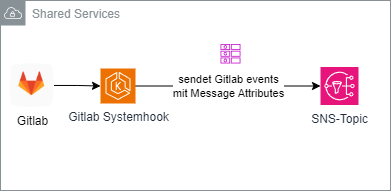
\includegraphics[scale=0.5]{systemhookOnly.drawio.png}
    \caption{Implementierung der GitLab Systemhook}
\end{figure}

Das \texttt{Hook}-Struct sowie die Initialisierung der erforderlichen Komponenten, wie dem \hyperlink{GitLabClient}{\textcolor{AOBlau}{GitLab-Client}} und dem \hyperlink{SNSClient}{\textcolor{AOBlau}{AWS SNS-Client}}, wurden gemäß den Anforderungen definiert. Der Endpunkt, an den die \hyperlink{HTTPPOST}{\textcolor{AOBlau}{HTTP-POST}}-Anfragen gesendet werden, ist \texttt{/api/v1/hook}. Dieser wird durch die Methode \texttt{handleHook} in der \texttt{Hook}-Struct verarbeitet, die im \Anhang{app:Test} dargestellt wird. Der Ablauf beginnt mit der Authentifizierung der \hyperlink{HTTP}{\textcolor{AOBlau}{HTTP-POST}}-Anfragen durch die Überprüfung des Tokens, um sicherzustellen, dass nur autorisierte Systeme Zugriff auf die \hyperlink{API}{\textcolor{AOBlau}{API}} erhalten. Codeauschnitte des Authentifizierung- prozesses befinden sich im \Anhang{app:CNMI}.

Sobald ein \hyperlink{GitLabEvent}{\textcolor{AOBlau}{GitLab Event}} erfasst wurde, erfolgt die Verarbeitung der \hyperlink{Payload}{\textcolor{AOBlau}{Payload}} asynchron. Durch die asynchrone Verarbeitung werden eingehende Anfragen schnell entgegengenommen und weiterverarbeitet, ohne das System zu blockieren. Im nächsten Schritt wird die empfangene Payload an den \hyperlink{SNS}{\textcolor{AOBlau}{SNS}}-Dienst gesendet\footnote{AWS - Amazon Simple Notification Service Documentation, \cite{aws2023sns}.}, wie in \Anhang{app:CNMI} veranschaulicht. Damit die Nachrichten gezielt gefiltert und ausgewertet werden können, werden sogenannte \hyperlink{MessageAttributes}{\textcolor{AOBlau}{Message Attributes}} erstellt. Diese Attribute enthalten Informationen über das jeweilige \hyperlink{GitLabEvent}{\textcolor{AOBlau}{Event}}, wie z.B. den Eventnamen oder spezifische Merkmale des Benutzers, der das Event ausgelöst hat. Im Falle einer Benutzererstellung wird beispielsweise geprüft, ob der neue Benutzer ein Bot ist, was ebenfalls als Attribut weitergeleitet wird.

Die \hyperlink{MessageAttributes}{\textcolor{AOBlau}{Message Attributes}} spielen eine entscheidende Rolle bei der Filterung und ermöglichen eine granulare Weiterleitung von \hyperlink{GitLabEvent}{\textcolor{AOBlau}{GitLab Events}}. Auf Basis dieser Attribute können spezifische \hyperlink{FilterPolicies}{\textcolor{AOBlau}{Filter Policies}} angewendet werden, sodass nur relevante \hyperlink{Events}{\textcolor{AOBlau}{Events}} an nachgelagerte Systeme oder Prozesse weitergeleitet werden.

\subsection{Implementierung des Dev-Kickstarter}
\label{sec:ImplementierungBenutzeroberflaeche}

Im Rahmen der Implementierung des Dev-Kickstarter wurde eine robuste Architektur entworfen, die es ermöglicht, \textbf{user\_create} Events zu verarbeiten und Aktionen wie das Versenden von Willkommens-E-Mails und das Hinzufügen neuer Benutzer zu \hyperlink{MicrosoftTeams}{\textcolor{AOBlau}{Microsoft Teams}}-Gruppen automatisiert auszuführen.


\begin{figure}[h!]
    \centering
    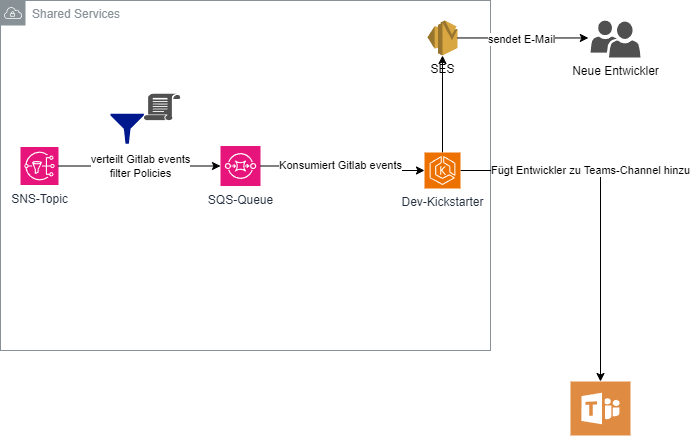
\includegraphics[scale=0.5]{dev-kickstarterOnly.drawio.png}
    \caption{Implementierung des Dev-Kickstarter}
\end{figure}

Das \texttt{Kickstarter}-Struct sowie die Initialisierung der erforderlichen Komponenten, wie dem \hyperlink{AWSSESClient}{\textcolor{AOBlau}{AWS SES-Client}}, \hyperlink{SQSConsumer}{\textcolor{AOBlau}{SQS-Consumer}} und \hyperlink{GraphClient}{\textcolor{AOBlau}{Microsoft Graph-Client}}, wurden gemäß den Anforderungen definiert. Der \hyperlink{SQSConsumer}{\textcolor{AOBlau}{SQS-Consumer}} empfängt Nachrichten aus einer \hyperlink{SQS}{\textcolor{AOBlau}{SQS Queues}}, die mit \hyperlink{FilterPolicies}{\textcolor{AOBlau}{Filter Policies}} erstellt wurde, um nur relevante Ereignisse zu verarbeiten.\footnote{AWS - Amazon Simple Queue Service Documentation, \cite{aws2023sqs}.} Die Definition der \texttt{Kickstarter}-Struct ist im \Anhang{app:kickStruct} zu finden.

Nach dem Empfang einer Nachricht wird die \hyperlink{Payload}{\textcolor{AOBlau}{Payload}} asynchron verarbeitet. Dabei wird die E-Mail-Adresse des Benutzers extrahiert, um eine Willkommens-E-Mail über den \hyperlink{AWSSESClient}{\textcolor{AOBlau}{AWS SES-Dienst}}\footnote{AWS - Amazon Simple Email Service Documentation, \cite{aws2023ses}.} zu versenden. Anschließend wird der Benutzer automatisch zu einer definierten \hyperlink{MicrosoftTeams}{\textcolor{AOBlau}{Microsoft Teams}}-Gruppe hinzugefügt, indem die \hyperlink{MicrosoftGraphAPI}{\textcolor{AOBlau}{Microsoft Graph API}} verwendet wird.
Der zugehörige Code befindet sich im \Anhang{app:kickMain}.

\subsection{Implementierung der E-Mail}
\label{sec:ImplementierungGeschaeftslogik}

Die E-Mail wurde als \hyperlink{HTML}{\textcolor{AOBlau}{HTML}}-Dokument erstellt, um sicherzustellen, dass sie auf verschiedenen Endgeräten und E-Mail-Clients korrekt angezeigt wird. Dabei wurde \hyperlink{CSS}{\textcolor{AOBlau}{inline CSS}} verwendet, da viele E-Mail-Clients externe \hyperlink{CSS}{\textcolor{AOBlau}{Stylesheets}} nicht vollständig unterstützen. Dies gewährleistet eine konsistente Darstellung der E-Mail auf allen Plattformen.\footnote{Hub Spot - The Ultimate Guide to Email Design, \cite{HubSpot}.}

Ein wichtiges Merkmal der Implementierung ist die dynamische Personalisierung der Inhalte. Dazu wurde der Platzhalter \texttt{\{\{.FirstName\}\}} eingefügt, um den Vornamen des Empfängers einzufügen. Dieser Wert wird zur Laufzeit gefüllt, indem der Code des Empfängers ausgewertet und der entsprechende Vorname dynamisch in die Vorlage eingefügt wird.

Zusätzlich wurden nützliche Ressourcen und Links in die E-Mail integriert, wie z.B. der Zugriff auf interne TUI-Plattformen wie  \hyperlink{Runway}{\textcolor{AOBlau}{Runway}} und \hyperlink{OneSource}{\textcolor{AOBlau}{OneSource}}, um den neuen Teammitgliedern den Einstieg zu erleichtern. Sicherheitsaspekte wurden ebenfalls berücksichtigt, indem Links zu den TUI-Sicherheitsrichtlinien eingebunden wurden. Dies unterstreicht die Wichtigkeit des sicheren Arbeitens innerhalb der Organisation.

Wie die finale E-Mail aussieht, kann im \Anhang{app:finalDesign} eingesehen werden.
